\section{Is the project V \& V approved?}
  V \& V refers to \textit{'Validation'} and \textit{'Verification'}. In this section I will discuss why I think this project is v \&
  v approved as well as discuss more about the deployment and testing of the new system.

  \begin{quote}
    \textit{'The aim of validation is to ensure that the software meets the customer's expectations'} [54]
  \end{quote}

  \begin{quote}
    \textit{'The aim of verification is to check that the software meets its stated functional and non-functional requirements'} [54]
  \end{quote}


  \subsection{Customer Feedback}
  To validate the product has met customer expectations, I think it's important to first note that the old system of phoning/emailing is still in 
  place for customers who don't want to transition to the new system. Systems on the web front-end could be put into place in the future to help 
  gain feedback of how the customer experience was and how it could be improved.

  In the previous report I spoke about how using the Agile software development lifecycle would also help keep customers/stakeholders involved in the 
  development process. This way of working also allows for quick changes, so if there ever is something inefficient or sub-standard with the service the 
  development team can quickly get to work at implementing the new changes.
  
  \subsection{Testing}
  \label{sec:Testing}

  When software is not tested issues such as poor quality, performance and user experience, security vulnerabilities and increased maintenance cost [55]
  can all occur.

  \begin{figure}[H]
    \centering
    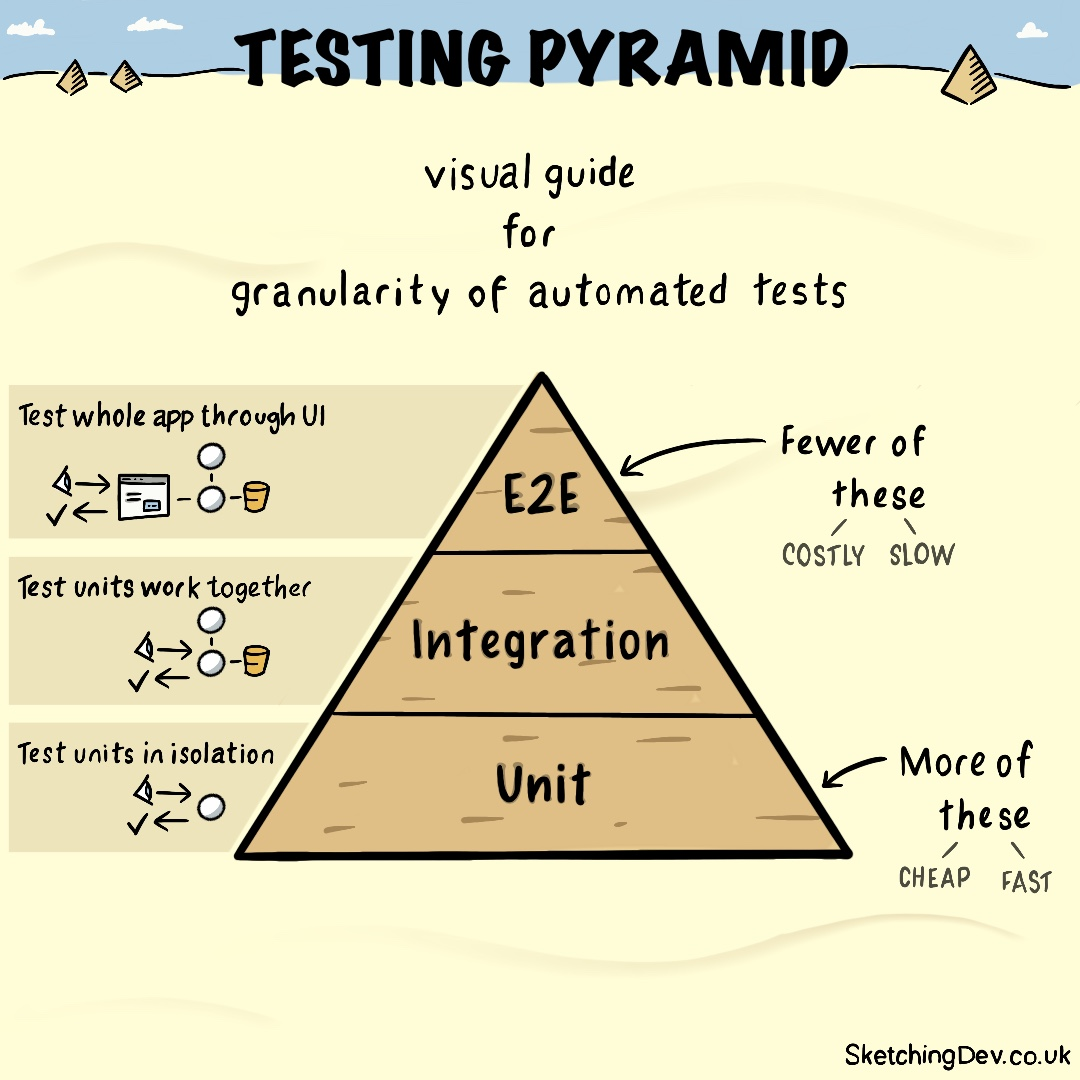
\includegraphics[width=10cm]{assets/testingPyramid.jpg}
    \caption{Image showing the testing pyramid, representing types of test and their quantity. [56]}
    \label{fig:testingPyramid}
  \end{figure}

  The testing pyramid above shows the types of testing ACME performs as well as demonstrates the quantity of each type of test.
  \begin{itemize}
    \item \textbf{Unit Tests} - These can be described as \textit{'consist[ing] in testing individual methods and functions of the classes, components, 
    or modules'} [57]. A simple example of a unit test would be to make sure a function that adds two number together, provides the expected result
    when given two numbers. Mocking, \textit{'replacement object for [a] dependency'} [58] are often used in these types of test to remain cheap by
    stopping expensive calls to databases or web requests by providing a pre-programmed response that the test can use instead. Due to their 
    lower cost unit tests can be ran before every deployment.

    \item \textbf{Integration Tests} - Unlike unit tests, integration tests want to test the actual functionality of the system, thus 
    making them more costly. In other words \textit{'Integration tests verify that different modules or services used by your application work well
    together'} [57]. These are run on a schedule rather than at deployment to help lower the overall expenditure of testing. 
  
    \item \textbf{End-to-end (E2E) Tests} - End-to-end tests, also known as UI tests, \textit{'replicates a user behavior with the software'} [57].
    This is done on software that is either live, or functions the exact same way the live system does. This is the most expensive type of testing as
    it often requires a large overhead to run. For example a library like Puppeteer [59] uses the chromium browser to make network requests to a 
    specified test url, then replicates user actions and runs assertions based on those actions. This is a lot more CPU intensive work than the 
    previous tests, and like integration tests should be run on a schedule.
  \end{itemize}

  A breakdown of ACMEs testing can be seen in \hyperref[sec:AppendixC]{\textbf{AppendixC}}.

  \subsection{Deployment}
  \label{sec:Deployment}

  Deployment can be described as the \textit{'process of putting software and software solutions into use or action'} [60]. This stage can be
  used to run tests, build and of course deploy the final application. Below is the jenkins pipeline ACME uses to deploy their app.

  \begin{figure}[H]
    \centering
    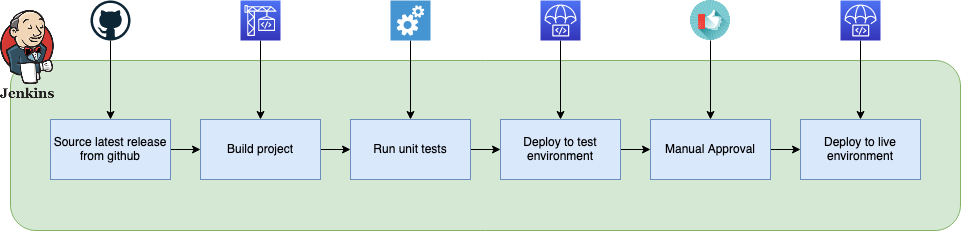
\includegraphics[width=12cm]{assets/relasePipeline.drawio.png}
    \caption{Diagram showing the stages of release for project.}
    \label{fig:releasePipeline}
  \end{figure}

  If at any point one of the stages fails, the pipeline fails and the following stages are not executed. This is helpful as if the unit tests fail this would
  indicate an issue and therefore we wouldn't want the broken system to be deployed to live. I have also set it up in a way where there are two environments.
  First the new code is deployed to test, where it can be double checked and made sure that it is ready by testers. Then, with manual approval, it can be 
  deployed to the live environment. The idea here is having this separation of environments will help catch bugs on the real hardware before going to live.

\newpage